O objetivo da pesquisa é caracterizar dimensões afetivas negativas em perfis do twitter localizando pontos comuns entre usúarios portadores de afetividades negativas (stress, ansiedade e depressão) de mesmo nível. Esse tipo de processo se asemelha com a aprendizagem não supervisionada, logo, antes dessa etapa é necessário mapearmos atributos, sendo assim, é necessário a identificação de usúarios com dimensões afetivas negativas em primeiro momento.

Como observado, existem vários passos para conclusão desse projeto, abertamente estrutura de processamento contára com um processo de mineração e dois processos de inteligencia artificial afim de gerar dois modelos lógicos. O primeiro modelo responsavel por inferir valores da EADS em um perfil, e o segundo, de predizer, a partir de dados do perfil, a probabilidade de existir um determinado nível de afetividade utilizando dados do perfil.

Projeto em geral tem alguns outros pontos sociais envolvidos, sendo um deles captação de dados embasados através de profissionais, entretando, nosso objetivo inicial é fazer a máquina coletar e acertar as previsões com qualquer tipo de dado (mesmo que fornercido por pessoas não capacitadas), sendo assim, detalharemos o sistema em si (coleta de dados e aprendizagem de maquina) e as metodologias utilizadas para desenvolve-lo.

Pode-se observar na Figura \ref{fig:tecnologias}, o sistema é divido em dois núcleos, o Dumont responsável por minerar e gerar toda a base de dados, e o 14BIS que será responsavel pelas Inteligencias Artificias.

\begin{figure}
    \centering
    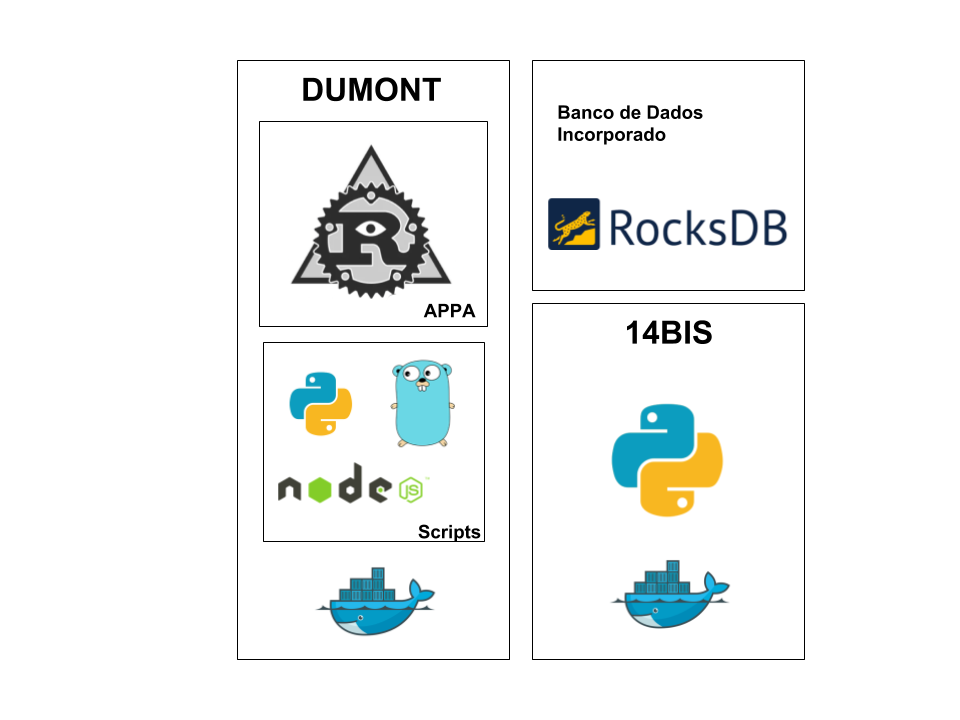
\includegraphics[width=1\textwidth]{imagens/tecnologias.png}
    \caption{Desenho apresentando os núcleos do projeto}
    \label{fig:tecnologias}
\end{figure}

Existem basicamente 5 técnologias que estão sendo utilizadas nesse projeto:
\begin{itemize}
 \item Python: É a linguagem atual mais utilizada no mundo de Aprendizado de Máquina, sua simplicidade ja á torna simples de usar, porém, a quantidade de materiais, bibliotecas e artigos sobre PLN e Aprendizado de Máquina á tornam a principal linguagem nesse projeto.
 \item Node/Javascript: Node é o interpretador que permite com que seja possivel executar o Javascript (linguagem originalmente de navegar no servidor). A linguagem tem um grande ganho com integrações e será utilizada para consumir recursos vindos de APIs.
 \item Go: Linguagem fortemente e estaticamente tipada, que fornecesse um poder de processamento equivalente a da linguagem C, entretando, muito mais simples de escrever e manter código, será utilizado para scripts onde serão necessário processamento de muitos dados.
 \item MongoDB: O Mongo é um banco não relacionado, em resumo, um grande banco de documentos indexados por atributos especificos, fornece um grande poder de leitura alem do fato de não ser prezo a estruturas pré-definidas como banco relacionais (isso facilita para que sejam inseridos novos dados futuramente sem grandes custos).
 \item Docker: Docker é uma ferramenta para infra-estrutura, será utilizado para rodar a aplicação em containers e facilitar o \textit{deploy}\footnote{Vindo do termo em inglês "lançar" é utilizado para o ato de colocar uma aplicação em ambiente de produção}.
\end{itemize}

Uma vez obtido conhecimento sobre os núcleos do projeto e suas técnologias, é possível idealizar o fluxo completo e interação entre elas. Se observar a Figura \ref{fig:tcc_caso_de_uso}, notara que o Dumont ira utilizar da API do twitter para coletar dados públicos, posteriormente esses dados serão processados e mutacionados a fim de gerar uma base de dados, por final essa base dados será salva em um banco de dados.

\begin{figure}
    \centering
    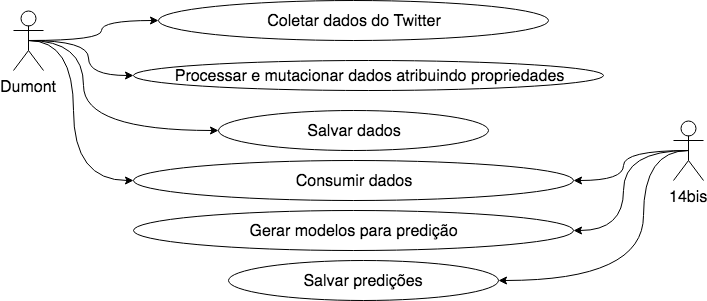
\includegraphics[width=.6\textwidth]{imagens/tcc_caso_de_uso.png}
    \caption{Diagrama de caso de uso do sistema}
    \label{fig:tcc_caso_de_uso}
\end{figure}

Revisando e reafirmando tudo o que foi dissertado até então, nosso objetivo é gerar uma base de conhecimento, aplica-la a uma aprendizagem supervisionada e em seguida aplicar esse dado a uma não supervisionada. Logo a primeira etapa é adquirir o \textit{dataset} que será utilizado.